\documentclass[fleqn,10pt]{wlscirep}
\usepackage[utf8]{inputenc}
\usepackage[T1]{fontenc}
\usepackage{amsmath,amssymb}
\DeclareMathOperator*{\SIGMA}{SIGMA}
\title{Opening Report of Crispr/Cas9-based Screening Data Analysis}

\author[1]{Y.Q. Yang}

%\keywords{Keyword1, Keyword2, Keyword3}

\begin{abstract}
In the opening report, I did a brief acadamic research on sgRNA specific pooled library screening, and part of current algorithms including MAGeCK and BAGEL.  Due to the difficulty of understanding these algorithm, I have problem finishing own-data analysis, which should be done in the work that follows. 
\end{abstract}
\begin{document}

\flushbottom
\maketitle
% * <john.hammersley@gmail.com> 2015-02-09T12:07:31.197Z:
%
%  Click the title above to edit the author information and abstract
%
\thispagestyle{empty}

%\noindent Please note: Abbreviations should be introduced at the first mention in the main text – no abbreviations lists. Suggested structure of main text (not enforced) is provided below.

\section*{Background}

In the first week of starting this project, I think it necessary for understanding what Crispr/Cas9-based genetic screening is, and what should be considered in analyzing the screening data.  The idea of Crispr/Cas9-based genetic screening was to use a pool of sgRNA-expressing lentivirus to generate a library of knockout cells that could be screened under both positive and negative selection. \cite{wang2014genetic} In addition to transfection, Pooled screening can avoid experimental errors caused by high expression of sgRNA.
However, the data generated by these screens pose several challenges to computational analysis. First, variance and statistical significance of comparisons between sample and control should be calculated under a extremely small sample size.  Second, different sgRNAs target the same gene might have different specificities and knockout efficiencies, which should be taken into account in the algorithm.  Third, the difference between read count distributions are significant, which calls for a robust normalization. \cite{li2014mageck}

\section*{Results}

Up to three levels of \textbf{subheading} are permitted. Subheadings should not be numbered.

\subsection*{Principles of MAGeCK Algorithm}

\subsubsection*{Overview of MAGeCK Algorithm}

A schematic of the MAGeCK Algorithm is presented as follow.
\begin{enumerate}
    \item Read counts from different samples are median-normalized, which enables each sample to have the same median value.
    \item A mean-variance model is established by following the \textbf{empirical} equation:
        \begin{equation}
           \hat{\sigma}^2=\hat{\mu}+k\hat{\mu}^b
        \end{equation}
    \end{enumerate}

\subsubsection*{Algorithm Characteristics}

This algorithm particularly uses a negative binomial(NB) model to test whether the sgRNA abboudance is significantly different between treatments and control based on the P-value calculated from the model\cite{li2014mageck}.  Considering that the sample size of sgRNA-specific pooled screening is relatively small and discrete, commonly used probablity distribution model such as binomial or Poisson, which is derived from large-sample asymptotic theory, may not appropriately model the count viability in RNA-Seq data.\cite{di2011nbp} Current RNA-Seq methods, including FPKM and TPM, which have been introduced in class, typically normalize data by scaling the number of reads in a given lane or library to a common value across all sequenced libraries in the experiment.  However, library size scaling is too simple for many biological conditions\cite{robinson2010scaling}.

\section*{Discussion}

The Discussion should be succinct and must not contain subheadings.

\section*{Methods}

Topical subheadings are allowed. Authors must ensure that their Methods section includes adequate experimental and characterization data necessary for others in the field to reproduce their work.

\bibliography{sample}

\noindent LaTeX formats citations and references automatically using the bibliography records in your .bib file, which you can edit via the project menu. Use the cite command for an inline citation, e.g. 

For data citations of datasets uploaded to e.g. \emph{figshare}, please use the \verb|howpublished| option in the bib entry to specify the platform and the link, as in the \verb|Hao:gidmaps:2014| example in the sample bibliography file.

\section*{Acknowledgements (not compulsory)}

Acknowledgements should be brief, and should not include thanks to anonymous referees and editors, or effusive comments. Grant or contribution numbers may be acknowledged.

\section*{Author contributions statement}

Must include all authors, identified by initials, for example:
A.A. conceived the experiment(s),  A.A. and B.A. conducted the experiment(s), C.A. and D.A. analysed the results.  All authors reviewed the manuscript. 

\section*{Additional information}

To include, in this order: \textbf{Accession codes} (where applicable); \textbf{Competing interests} (mandatory statement). 

The corresponding author is responsible for submitting a \href{http://www.nature.com/srep/policies/index.html#competing}{competing interests statement} on behalf of all authors of the paper. This statement must be included in the submitted article file.

\begin{figure}[ht]
\centering
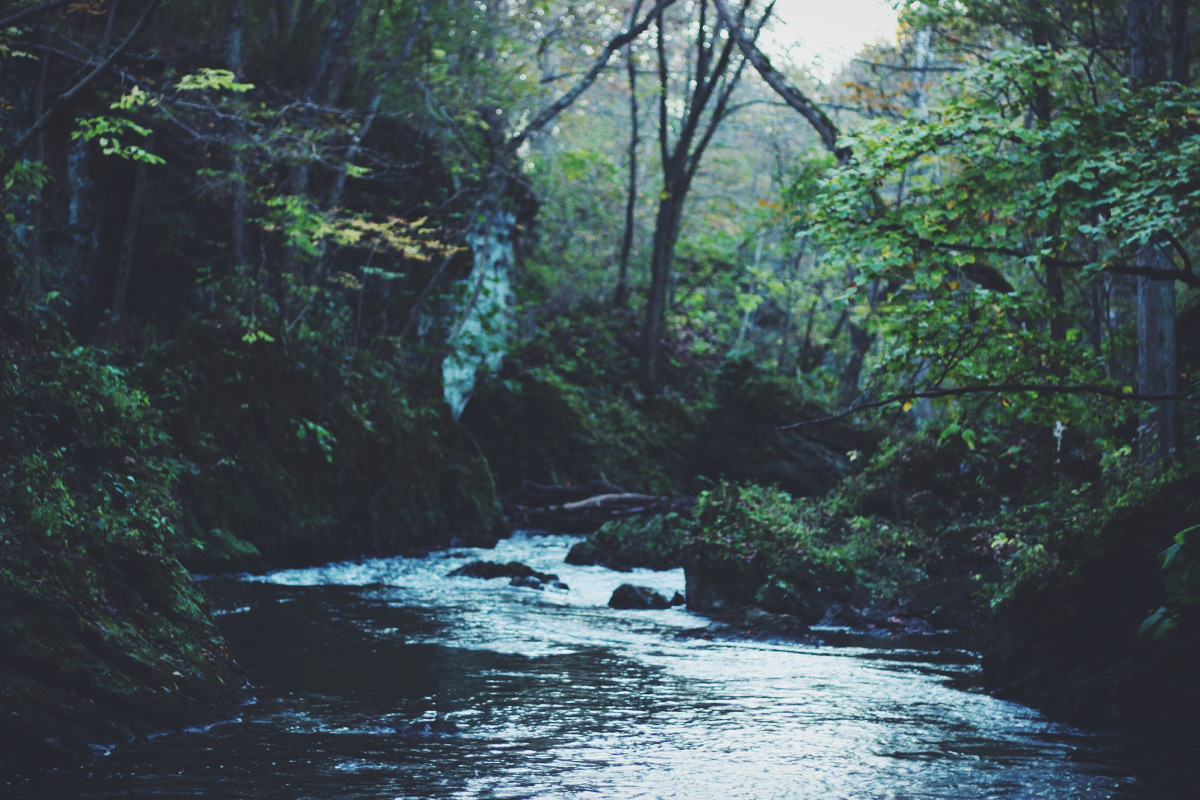
\includegraphics[width=\linewidth]{stream}
\caption{Legend (350 words max). Example legend text.}
\label{fig:stream}
\end{figure}

\begin{table}[ht]
\centering
\begin{tabular}{|l|l|l|}
\hline
Condition & n & p \\
\hline
A & 5 & 0.1 \\
\hline
B & 10 & 0.01 \\
\hline
\end{tabular}
\caption{\label{tab:example}Legend (350 words max). Example legend text.}
\end{table}

Figures and tables can be referenced in LaTeX using the ref command, e.g. Figure \ref{fig:stream} and Table \ref{tab:example}.

\end{document}